\section{Physical Connections and Interfaces}

`v3 sensor boards and rain gauge' means a set of sensors which includs a v3.1 Metsense board, a v3.1 Lightsense board, a Chemsense board, and Rain Gauge.
In this section, we will only deal with physical connection between Rain Gauge and Metsense board.
\par

Physical connections between a Metsense board and a rain gauge are shown in the Figure \ref{fig:connect}. A rain gauge is connected to Metsense board directly through wires. The connection between the rain gauge and Metsense board is detected through an analog read signal through pin 2 of 3V3AD. When zero voltage, ground, is connected to Pin 2 of 3V3AD, sensor board notice that a rain gauge is connected. Therefore, the ground line from rain gauge need to be connected to both pin 1, which is ground, and 2 of 3V3AD simultaneously. The rain gauge deliver data through pin 2 of JP2, digital up/down signal.



\begin{figure}[h]
\begin{center}
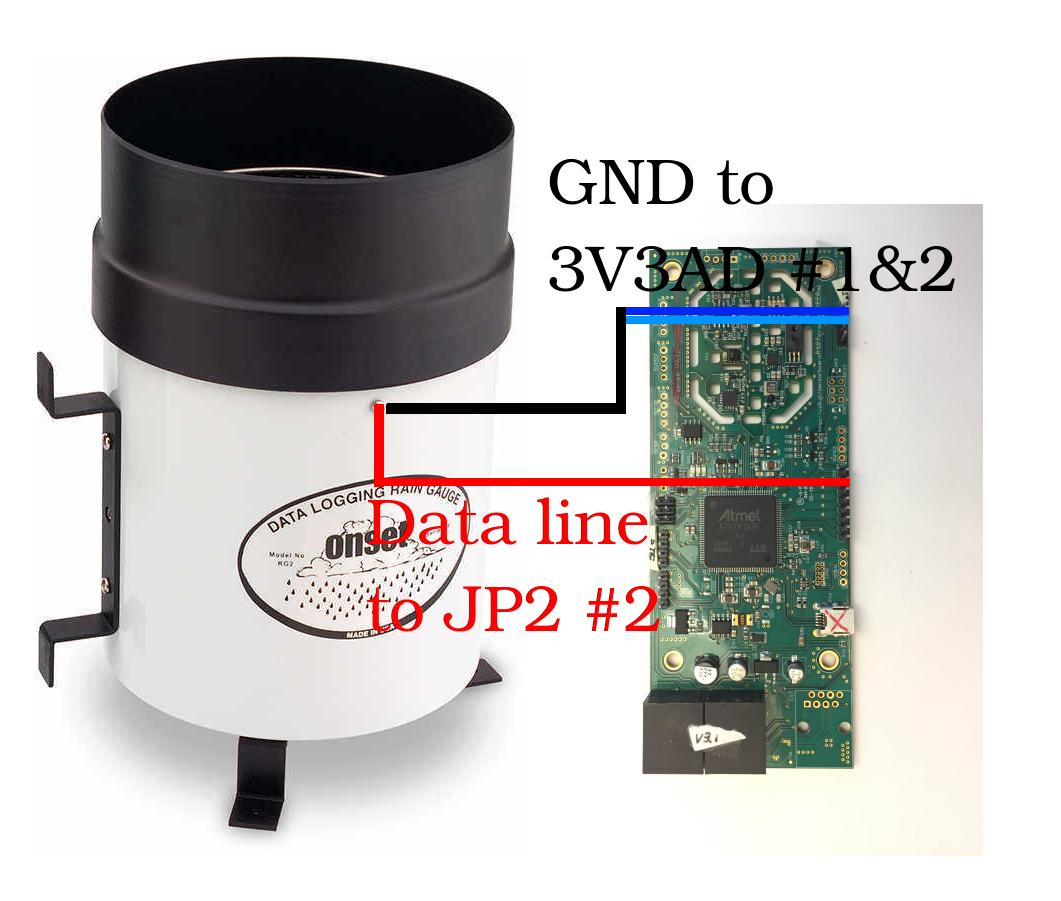
\includegraphics[width=4in]{con.png}
\caption{Connections between a Metsense board and a rain gauge}
\label{fig:connect}
\end{center}
\end{figure}

Detail wireing to the rain gauge and board is shown in Figure \ref{fig:gauge_in} - \ref{fig:gauge_board}. Wire from the rain gauge as shown in Figure \ref{fig:gauge_in} is going out though a hole of the body of the rain gauge as shown in Figure \ref{fig:gauge_out}, and connected to the board as shown in Figure \ref{fig:connect}. Before the two lines from the rain gauge are connected to the Metsense board, the ground line need to be distinguished. You can use a multimeter to find one. Set a multimeter to measure voltage, connect each of the line to probes of the multimeter and move a tick inside of the rain gauge. Then you can tell which one is ground.
\par
Pin detail of the Metsense board is shown in Figure \ref{fig:gauge_board}. Deep blue squre marked in Figure \ref{fig:gauge_board} is a ground pin, and light blue squre is a connection pin. The connection pin and gound line of rain gauge need to be connected to the ground pin. Data pin marked as a red squre need to be connected to data line of rain gauge.


\makeatletter
\setlength{\@fptop}{0pt}
\makeatother


\begin{figure}[!htb]
\minipage{0.32\textwidth}
  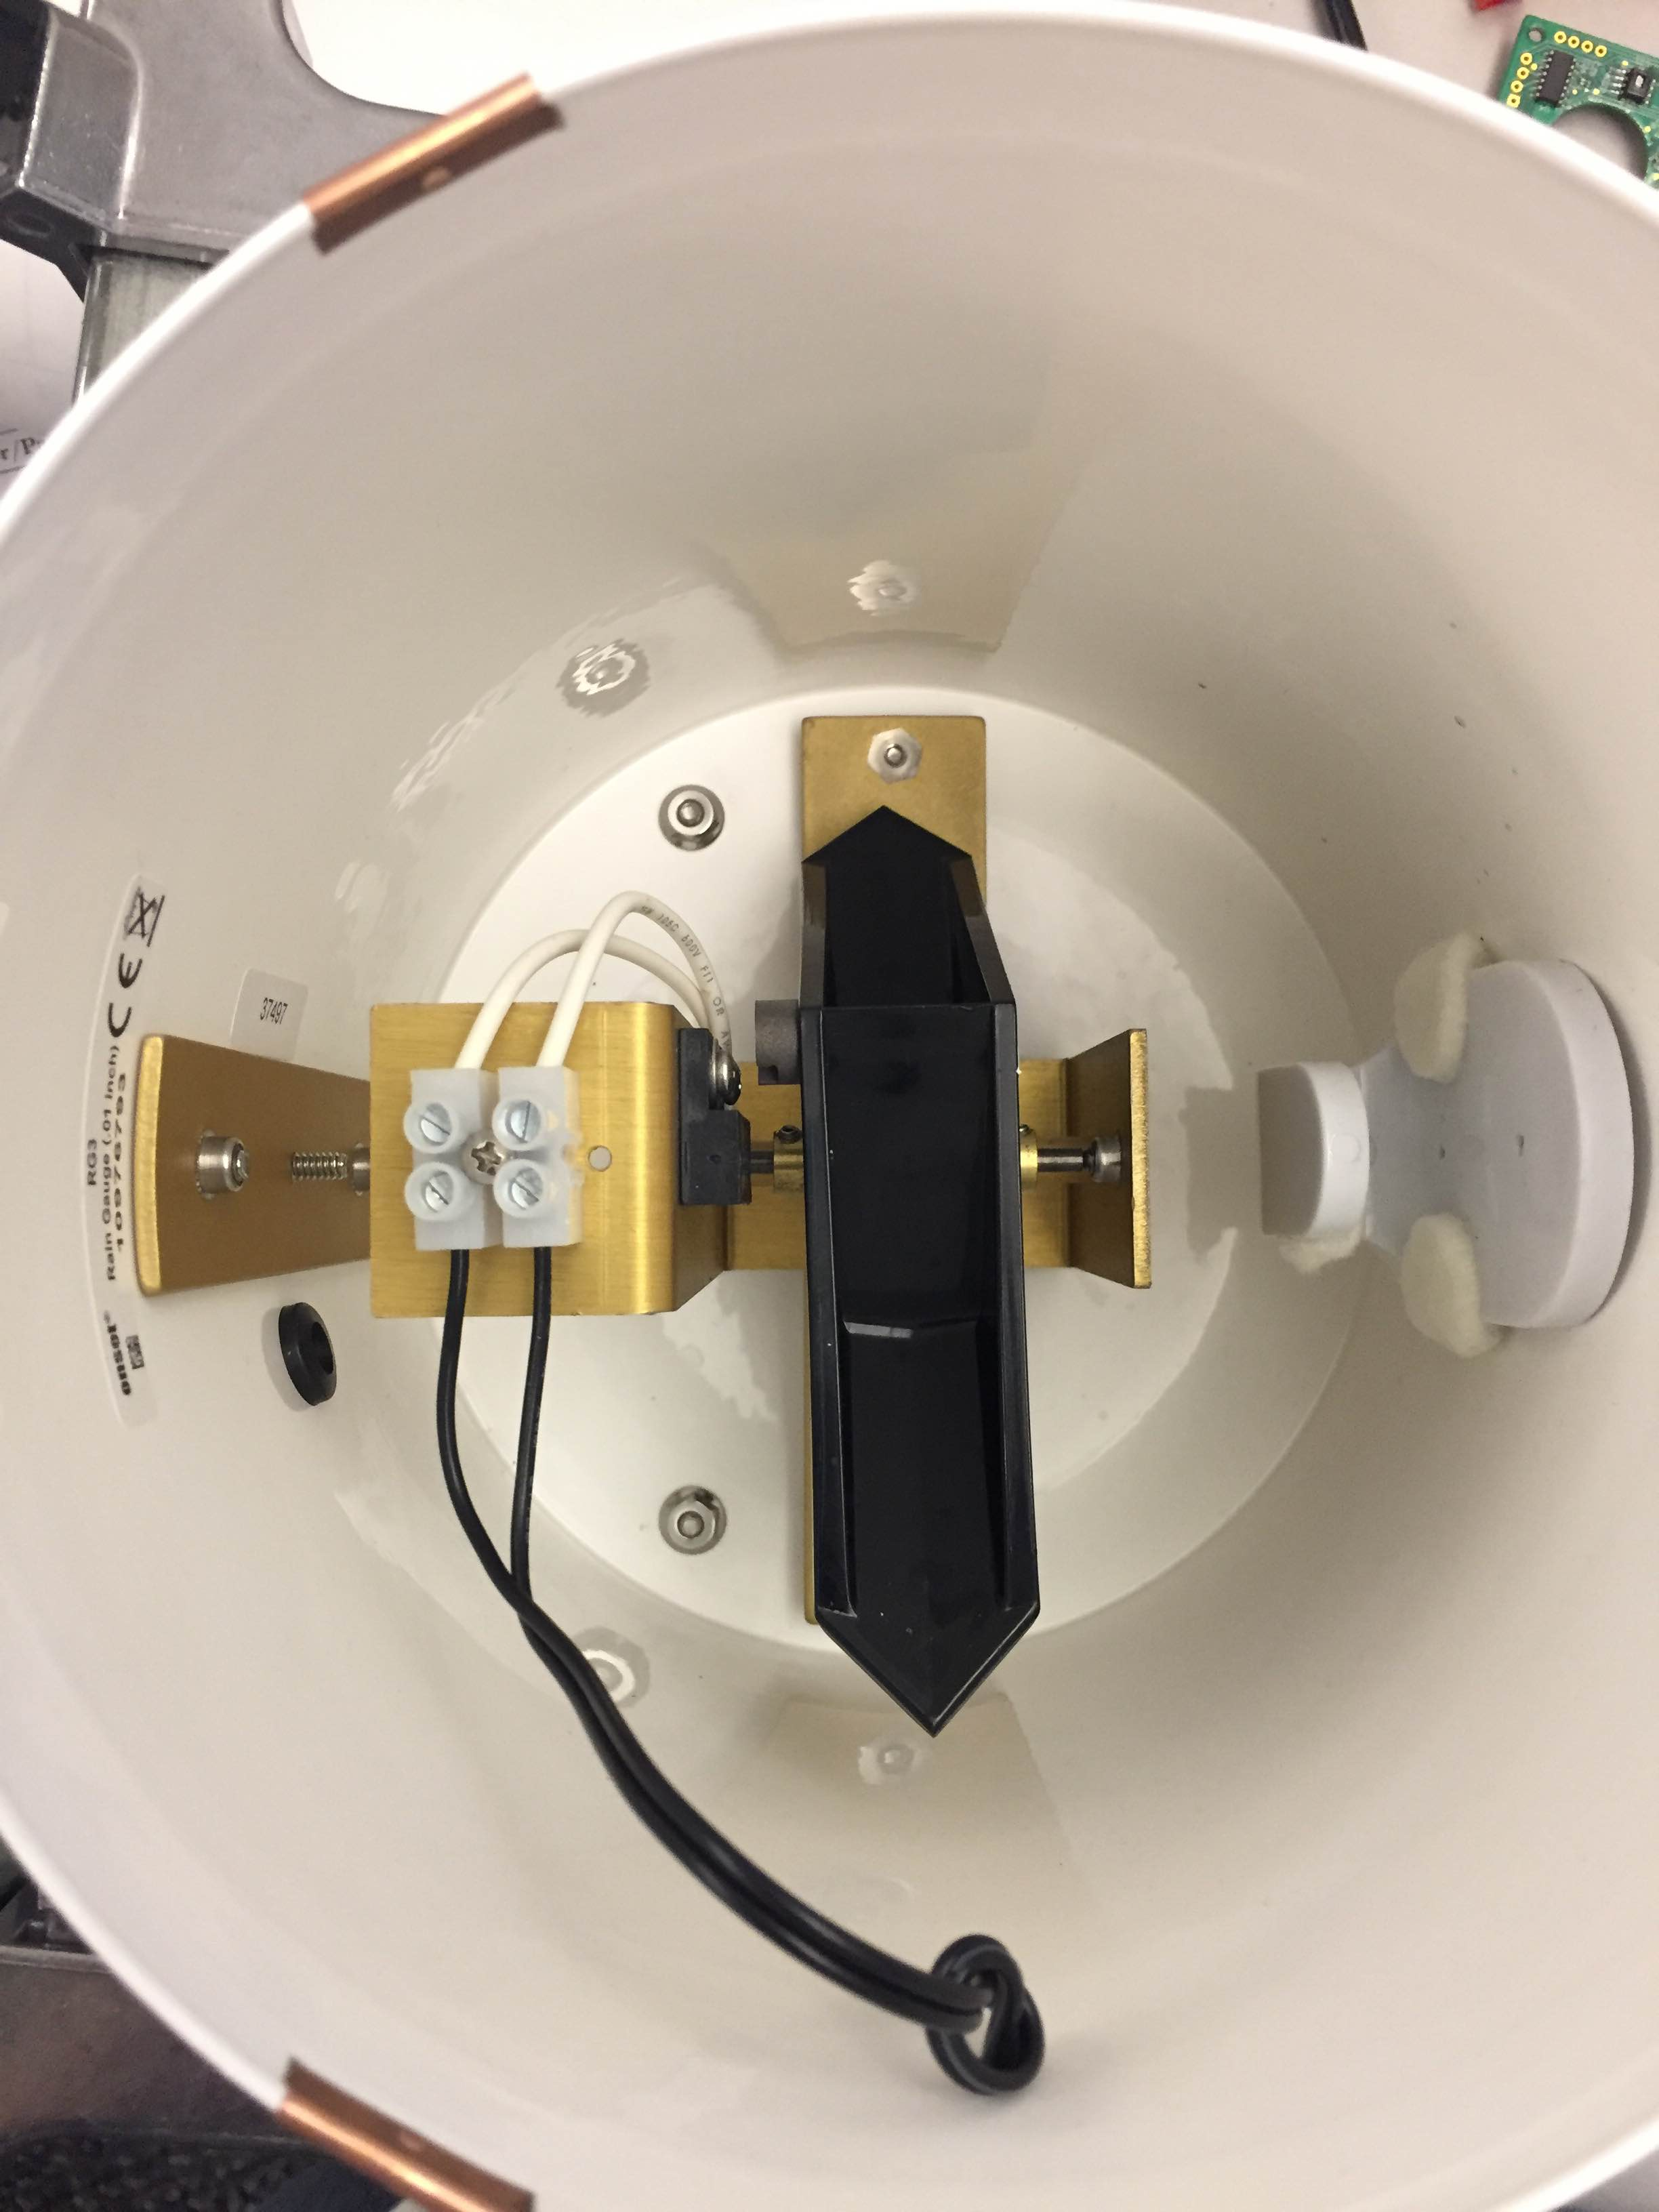
\includegraphics[width=\linewidth]{in.png}
  \caption{Connections inside of the rain gauge}
  \label{fig:gauge_in}
\endminipage\hfill
\minipage{0.32\textwidth}
  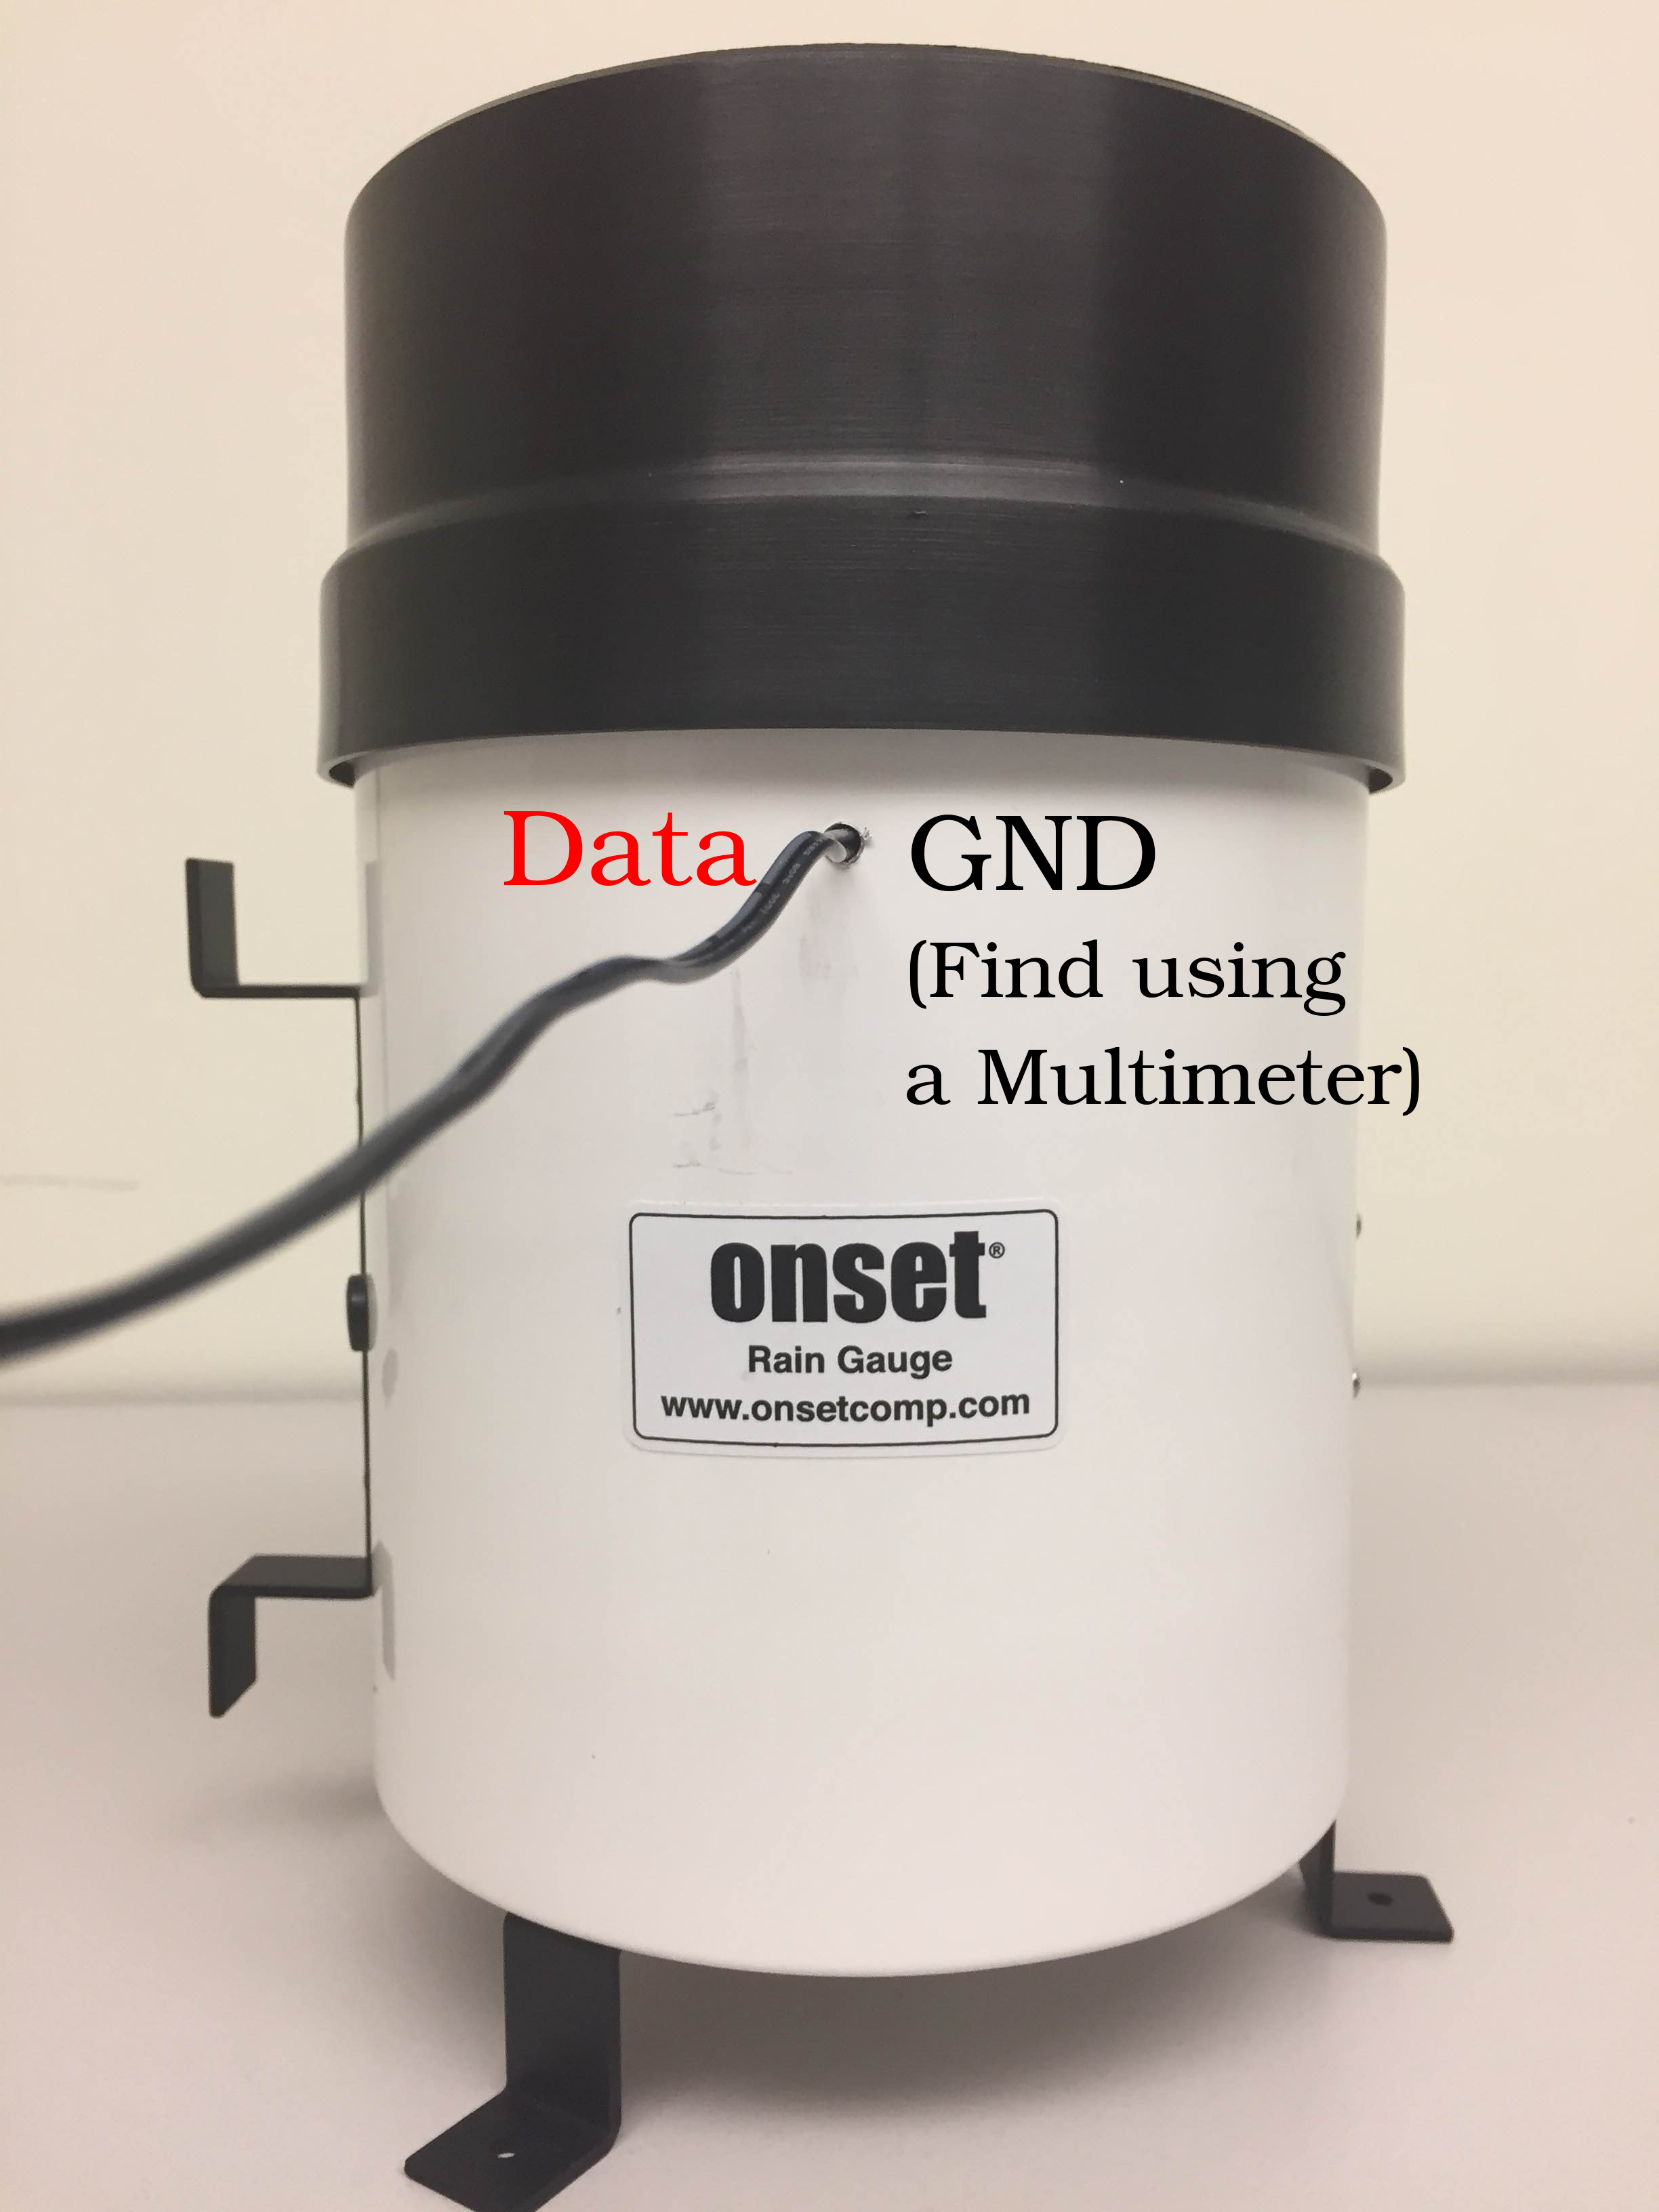
\includegraphics[width=\linewidth]{gauge.png}
  \caption{Connections outside of the rain gause}
  \label{fig:gauge_out}
\endminipage\hfill
\minipage{0.32\textwidth}%
  \includegraphics[width=\linewidth]{a.png}
  \caption{Connections to the Metsense board}
  \label{fig:gauge_board}
\endminipage
\end{figure}

\clearpage